% Options for packages loaded elsewhere
\PassOptionsToPackage{unicode}{hyperref}
\PassOptionsToPackage{hyphens}{url}
%
\documentclass[
]{article}
\usepackage{amsmath,amssymb}
\usepackage{iftex}
\ifPDFTeX
  \usepackage[T1]{fontenc}
  \usepackage[utf8]{inputenc}
  \usepackage{textcomp} % provide euro and other symbols
\else % if luatex or xetex
  \usepackage{unicode-math} % this also loads fontspec
  \defaultfontfeatures{Scale=MatchLowercase}
  \defaultfontfeatures[\rmfamily]{Ligatures=TeX,Scale=1}
\fi
\usepackage{lmodern}
\ifPDFTeX\else
  % xetex/luatex font selection
\fi
% Use upquote if available, for straight quotes in verbatim environments
\IfFileExists{upquote.sty}{\usepackage{upquote}}{}
\IfFileExists{microtype.sty}{% use microtype if available
  \usepackage[]{microtype}
  \UseMicrotypeSet[protrusion]{basicmath} % disable protrusion for tt fonts
}{}
\makeatletter
\@ifundefined{KOMAClassName}{% if non-KOMA class
  \IfFileExists{parskip.sty}{%
    \usepackage{parskip}
  }{% else
    \setlength{\parindent}{0pt}
    \setlength{\parskip}{6pt plus 2pt minus 1pt}}
}{% if KOMA class
  \KOMAoptions{parskip=half}}
\makeatother
\usepackage{xcolor}
\usepackage[margin=1in]{geometry}
\usepackage{color}
\usepackage{fancyvrb}
\newcommand{\VerbBar}{|}
\newcommand{\VERB}{\Verb[commandchars=\\\{\}]}
\DefineVerbatimEnvironment{Highlighting}{Verbatim}{commandchars=\\\{\}}
% Add ',fontsize=\small' for more characters per line
\usepackage{framed}
\definecolor{shadecolor}{RGB}{248,248,248}
\newenvironment{Shaded}{\begin{snugshade}}{\end{snugshade}}
\newcommand{\AlertTok}[1]{\textcolor[rgb]{0.94,0.16,0.16}{#1}}
\newcommand{\AnnotationTok}[1]{\textcolor[rgb]{0.56,0.35,0.01}{\textbf{\textit{#1}}}}
\newcommand{\AttributeTok}[1]{\textcolor[rgb]{0.13,0.29,0.53}{#1}}
\newcommand{\BaseNTok}[1]{\textcolor[rgb]{0.00,0.00,0.81}{#1}}
\newcommand{\BuiltInTok}[1]{#1}
\newcommand{\CharTok}[1]{\textcolor[rgb]{0.31,0.60,0.02}{#1}}
\newcommand{\CommentTok}[1]{\textcolor[rgb]{0.56,0.35,0.01}{\textit{#1}}}
\newcommand{\CommentVarTok}[1]{\textcolor[rgb]{0.56,0.35,0.01}{\textbf{\textit{#1}}}}
\newcommand{\ConstantTok}[1]{\textcolor[rgb]{0.56,0.35,0.01}{#1}}
\newcommand{\ControlFlowTok}[1]{\textcolor[rgb]{0.13,0.29,0.53}{\textbf{#1}}}
\newcommand{\DataTypeTok}[1]{\textcolor[rgb]{0.13,0.29,0.53}{#1}}
\newcommand{\DecValTok}[1]{\textcolor[rgb]{0.00,0.00,0.81}{#1}}
\newcommand{\DocumentationTok}[1]{\textcolor[rgb]{0.56,0.35,0.01}{\textbf{\textit{#1}}}}
\newcommand{\ErrorTok}[1]{\textcolor[rgb]{0.64,0.00,0.00}{\textbf{#1}}}
\newcommand{\ExtensionTok}[1]{#1}
\newcommand{\FloatTok}[1]{\textcolor[rgb]{0.00,0.00,0.81}{#1}}
\newcommand{\FunctionTok}[1]{\textcolor[rgb]{0.13,0.29,0.53}{\textbf{#1}}}
\newcommand{\ImportTok}[1]{#1}
\newcommand{\InformationTok}[1]{\textcolor[rgb]{0.56,0.35,0.01}{\textbf{\textit{#1}}}}
\newcommand{\KeywordTok}[1]{\textcolor[rgb]{0.13,0.29,0.53}{\textbf{#1}}}
\newcommand{\NormalTok}[1]{#1}
\newcommand{\OperatorTok}[1]{\textcolor[rgb]{0.81,0.36,0.00}{\textbf{#1}}}
\newcommand{\OtherTok}[1]{\textcolor[rgb]{0.56,0.35,0.01}{#1}}
\newcommand{\PreprocessorTok}[1]{\textcolor[rgb]{0.56,0.35,0.01}{\textit{#1}}}
\newcommand{\RegionMarkerTok}[1]{#1}
\newcommand{\SpecialCharTok}[1]{\textcolor[rgb]{0.81,0.36,0.00}{\textbf{#1}}}
\newcommand{\SpecialStringTok}[1]{\textcolor[rgb]{0.31,0.60,0.02}{#1}}
\newcommand{\StringTok}[1]{\textcolor[rgb]{0.31,0.60,0.02}{#1}}
\newcommand{\VariableTok}[1]{\textcolor[rgb]{0.00,0.00,0.00}{#1}}
\newcommand{\VerbatimStringTok}[1]{\textcolor[rgb]{0.31,0.60,0.02}{#1}}
\newcommand{\WarningTok}[1]{\textcolor[rgb]{0.56,0.35,0.01}{\textbf{\textit{#1}}}}
\usepackage{graphicx}
\makeatletter
\def\maxwidth{\ifdim\Gin@nat@width>\linewidth\linewidth\else\Gin@nat@width\fi}
\def\maxheight{\ifdim\Gin@nat@height>\textheight\textheight\else\Gin@nat@height\fi}
\makeatother
% Scale images if necessary, so that they will not overflow the page
% margins by default, and it is still possible to overwrite the defaults
% using explicit options in \includegraphics[width, height, ...]{}
\setkeys{Gin}{width=\maxwidth,height=\maxheight,keepaspectratio}
% Set default figure placement to htbp
\makeatletter
\def\fps@figure{htbp}
\makeatother
\setlength{\emergencystretch}{3em} % prevent overfull lines
\providecommand{\tightlist}{%
  \setlength{\itemsep}{0pt}\setlength{\parskip}{0pt}}
\setcounter{secnumdepth}{-\maxdimen} % remove section numbering
\usepackage{fontspec}
\setmainfont{Times New Roman}
\usepackage{ctex}
\ifLuaTeX
  \usepackage{selnolig}  % disable illegal ligatures
\fi
\usepackage{bookmark}
\IfFileExists{xurl.sty}{\usepackage{xurl}}{} % add URL line breaks if available
\urlstyle{same}
\hypersetup{
  pdftitle={homework3},
  pdfauthor={黄舟翔 3220103606},
  hidelinks,
  pdfcreator={LaTeX via pandoc}}

\title{homework3}
\author{黄舟翔 3220103606}
\date{2025-06-28}

\begin{document}
\maketitle

\textbf{Background}: In the previous lectures and lab, we fitted the
following model \[
 Y = y_0 N^a + \mathrm{noise}
\] by minimizing the mean squared error \[
 \frac{1}{n}\sum_{i=1}^{n}{(Y_i - y_0 N_i^a)^2}.
\]

We did this by approximating the derivative of the MSE, and adjusting
\(a\) by an amount proportional to that, stopping when the derivative
became small. Our procedure assumed we knew \(y_0\). In this assignment,
we will use a built-in R function to estimate both parameters at once;
it uses a fancier version of the same idea.

Because the model is nonlinear, there is no simple formula for the
parameter estimates in terms of the data. Also unlike linear models,
there is no simple formula for the \emph{standard errors} of the
parameter estimates. We will therefore use a technique called
\textbf{the jackknife} to get approximate standard errors.

Here is how the jackknife works:

\begin{itemize}
\tightlist
\item
  Get a set of \(n\) data points and get an estimate \(\hat{\theta}\)
  for the parameter of interest \(\theta\).
\item
  For each data point \(i\), remove \(i\) from the data set, and get an
  estimate \(\hat{\theta}_{(-i)}\) from the remaining \(n-1\) data
  points. The \(\hat{\theta}_{(-i)}\) are sometimes called the
  ``jackknife estimates''.
\item
  Find the mean \(\overline{\theta}\) of the \(n\) values of
  \(\hat{\theta}_{(-i)}\)
\item
  The jackknife variance of \(\hat{\theta}\) is \[
  \frac{n-1}{n}\sum_{i=1}^{n}{(\hat{\theta}_{(-i)} - \overline{\theta})^2} = \frac{(n-1)^2}{n}\mathrm{var}{[\hat{\theta}_{(-i)}]}
  \] where \(\mathrm{var}\) stands for the sample variance.
  (\emph{Challenge}: can you explain the factor of \((n-1)^2/n\)?
  \emph{Hint}: think about what happens when \(n\) is large so
  \((n-1)/n \approx 1\).)
\item
  The jackknife standard error of \(\hat{\theta}\) is the square root of
  the jackknife variance.
\end{itemize}

You will estimate the power-law scaling model, and its uncertainty,
using the data alluded to in lecture, available in the file
\texttt{gmp.dat} from lecture, which contains data for 2006.

\begin{verbatim}
gmp <- read.table("gmp.dat")
gmp$pop <- round(gmp$gmp/gmp$pcgmp)
\end{verbatim}

\subsubsection{1.}\label{section}

First, plot the data as in lecture, with per capita GMP on the y-axis
and population on the x-axis. Add the curve function with the default
values provided in lecture. Add two more curves corresponding to
\(a=0.1\) and \(a=0.15\); use the \texttt{col} option to give each curve
a different color (of your choice).

用以下代码完成

\begin{Shaded}
\begin{Highlighting}[]
\NormalTok{gmp }\OtherTok{\textless{}{-}} \FunctionTok{read.table}\NormalTok{(}\StringTok{"data/gmp.dat"}\NormalTok{, }\AttributeTok{col.names =} \FunctionTok{c}\NormalTok{(}\StringTok{"MSA"}\NormalTok{, }\StringTok{"gmp"}\NormalTok{, }\StringTok{"pcgmp"}\NormalTok{))}
\NormalTok{gmp}\SpecialCharTok{$}\NormalTok{pop }\OtherTok{\textless{}{-}} \FunctionTok{round}\NormalTok{(gmp}\SpecialCharTok{$}\NormalTok{gmp }\SpecialCharTok{/}\NormalTok{ gmp}\SpecialCharTok{$}\NormalTok{pcgmp)}

\CommentTok{\# 绘制散点图}
\FunctionTok{plot}\NormalTok{(pcgmp }\SpecialCharTok{\textasciitilde{}}\NormalTok{ pop, }\AttributeTok{data =}\NormalTok{ gmp, }\AttributeTok{log =} \StringTok{"xy"}\NormalTok{, }
     \AttributeTok{xlab =} \StringTok{"Population"}\NormalTok{, }\AttributeTok{ylab =} \StringTok{"Per Capita GMP"}\NormalTok{,}
     \AttributeTok{main =} \StringTok{"Power Law Scaling (2006)"}\NormalTok{)}

\CommentTok{\# 添加三条理论曲线}
\FunctionTok{curve}\NormalTok{(}\DecValTok{6611} \SpecialCharTok{*}\NormalTok{ x}\SpecialCharTok{\^{}}\NormalTok{(}\DecValTok{1}\SpecialCharTok{/}\DecValTok{8}\NormalTok{), }\AttributeTok{add =} \ConstantTok{TRUE}\NormalTok{, }\AttributeTok{col =} \StringTok{"blue"}\NormalTok{, }\AttributeTok{lwd =} \DecValTok{2}\NormalTok{)      }\CommentTok{\# 默认值}
\FunctionTok{curve}\NormalTok{(}\DecValTok{5000} \SpecialCharTok{*}\NormalTok{ x}\SpecialCharTok{\^{}}\FloatTok{0.10}\NormalTok{, }\AttributeTok{add =} \ConstantTok{TRUE}\NormalTok{, }\AttributeTok{col =} \StringTok{"red"}\NormalTok{, }\AttributeTok{lwd =} \DecValTok{2}\NormalTok{)        }\CommentTok{\# a=0.1}
\FunctionTok{curve}\NormalTok{(}\DecValTok{6611} \SpecialCharTok{*}\NormalTok{ x}\SpecialCharTok{\^{}}\FloatTok{0.15}\NormalTok{, }\AttributeTok{add =} \ConstantTok{TRUE}\NormalTok{, }\AttributeTok{col =} \StringTok{"darkgreen"}\NormalTok{, }\AttributeTok{lwd =} \DecValTok{2}\NormalTok{)  }\CommentTok{\# a=0.15}
\FunctionTok{legend}\NormalTok{(}\StringTok{"topright"}\NormalTok{, }\AttributeTok{legend =} \FunctionTok{c}\NormalTok{(}\StringTok{"y0=6611, a=0.125"}\NormalTok{, }\StringTok{"y0=5000, a=0.10"}\NormalTok{, }\StringTok{"y0=6611, a=0.15"}\NormalTok{),}
       \AttributeTok{col =} \FunctionTok{c}\NormalTok{(}\StringTok{"blue"}\NormalTok{, }\StringTok{"red"}\NormalTok{, }\StringTok{"darkgreen"}\NormalTok{), }\AttributeTok{lwd =} \DecValTok{2}\NormalTok{)}
\end{Highlighting}
\end{Shaded}

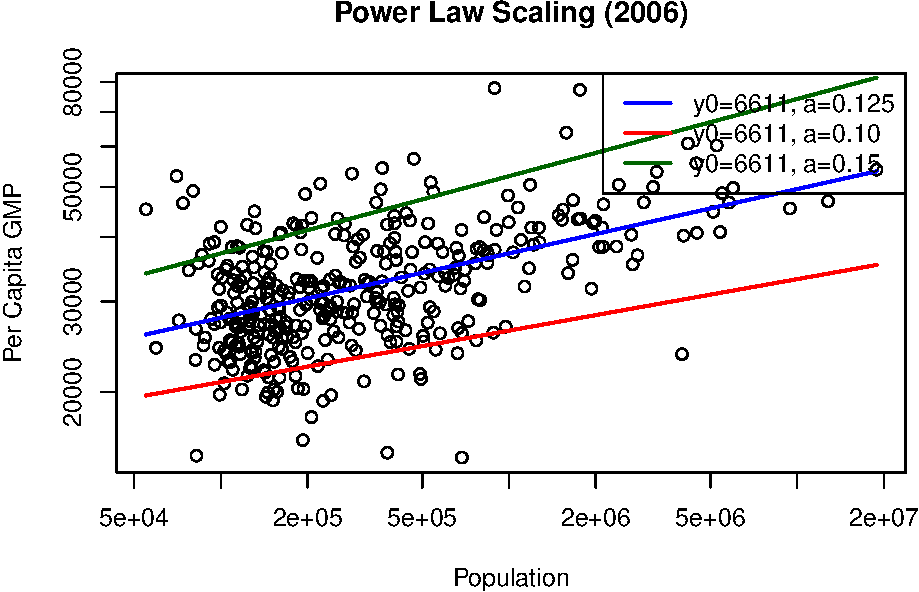
\includegraphics{Homework-03_files/figure-latex/unnamed-chunk-1-1.pdf}

\subsubsection{2.}\label{section-1}

Write a function, called \texttt{mse()}, which calculates the mean
squared error of the model on a given data set. \texttt{mse()} should
take three arguments: a numeric vector of length two, the first
component standing for \(y_0\) and the second for \(a\); a numerical
vector containing the values of \(N\); and a numerical vector containing
the values of \(Y\). The function should return a single numerical
value. The latter two arguments should have as the default values the
columns \texttt{pop} and \texttt{pcgmp} (respectively) from the
\texttt{gmp} data frame from lecture. Your function may not use
\texttt{for()} or any other loop. Check that, with the default data, you
get the following values.

用以下代码解决,经验证输出符合预期。

\begin{Shaded}
\begin{Highlighting}[]
\NormalTok{mse }\OtherTok{\textless{}{-}} \ControlFlowTok{function}\NormalTok{(params, }\AttributeTok{N =}\NormalTok{ gmp}\SpecialCharTok{$}\NormalTok{pop, }\AttributeTok{Y =}\NormalTok{ gmp}\SpecialCharTok{$}\NormalTok{pcgmp) \{}
\NormalTok{  y0 }\OtherTok{\textless{}{-}}\NormalTok{ params[}\DecValTok{1}\NormalTok{]}
\NormalTok{  a }\OtherTok{\textless{}{-}}\NormalTok{ params[}\DecValTok{2}\NormalTok{]}
\NormalTok{  predictions }\OtherTok{\textless{}{-}}\NormalTok{ y0 }\SpecialCharTok{*}\NormalTok{ (N}\SpecialCharTok{\^{}}\NormalTok{a)}
  \FunctionTok{mean}\NormalTok{((Y }\SpecialCharTok{{-}}\NormalTok{ predictions)}\SpecialCharTok{\^{}}\DecValTok{2}\NormalTok{)}
\NormalTok{\}}

\CommentTok{\# 验证函数输出}
\FunctionTok{mse}\NormalTok{(}\FunctionTok{c}\NormalTok{(}\DecValTok{6611}\NormalTok{, }\FloatTok{0.15}\NormalTok{))  }\CommentTok{\# 应返回 \textasciitilde{}207057513}
\end{Highlighting}
\end{Shaded}

\begin{verbatim}
## [1] 207057513
\end{verbatim}

\begin{Shaded}
\begin{Highlighting}[]
\FunctionTok{mse}\NormalTok{(}\FunctionTok{c}\NormalTok{(}\DecValTok{5000}\NormalTok{, }\FloatTok{0.10}\NormalTok{))  }\CommentTok{\# 应返回 \textasciitilde{}298459915}
\end{Highlighting}
\end{Shaded}

\begin{verbatim}
## [1] 298459914
\end{verbatim}

\begin{verbatim}
> mse(c(6611,0.15))
[1] 207057513
> mse(c(5000,0.10))
[1] 298459915
\end{verbatim}

\subsubsection{3.}\label{section-2}

R has several built-in functions for optimization, which we will meet as
we go through the course. One of the simplest is \texttt{nlm()}, or
non-linear minimization. \texttt{nlm()} takes two required arguments: a
function, and a starting value for that function. Run \texttt{nlm()}
three times with your function \texttt{mse()} and three starting value
pairs for \(y0\) and \(a\) as in

\begin{verbatim}
nlm(mse, c(y0=6611,a=1/8))
\end{verbatim}

What do the quantities \texttt{minimum} and \texttt{estimate} represent?
What values does it return for these?

用以下代码解决, minimum表示最小化的MSE值,estimate:表示参数估计值(y0, a)

\begin{Shaded}
\begin{Highlighting}[]
\NormalTok{fit1 }\OtherTok{\textless{}{-}} \FunctionTok{nlm}\NormalTok{(mse, }\FunctionTok{c}\NormalTok{(}\AttributeTok{y0 =} \DecValTok{6611}\NormalTok{, }\AttributeTok{a =} \DecValTok{1}\SpecialCharTok{/}\DecValTok{8}\NormalTok{))}
\NormalTok{fit2 }\OtherTok{\textless{}{-}} \FunctionTok{nlm}\NormalTok{(mse, }\FunctionTok{c}\NormalTok{(}\AttributeTok{y0 =} \DecValTok{6611}\NormalTok{, }\AttributeTok{a =} \FloatTok{0.15}\NormalTok{))}
\NormalTok{fit3 }\OtherTok{\textless{}{-}} \FunctionTok{nlm}\NormalTok{(mse, }\FunctionTok{c}\NormalTok{(}\AttributeTok{y0 =} \DecValTok{5000}\NormalTok{, }\AttributeTok{a =} \FloatTok{0.10}\NormalTok{))}

\CommentTok{\# 解释结果:}

\FunctionTok{list}\NormalTok{(}
  \AttributeTok{fit1 =} \FunctionTok{list}\NormalTok{(}\AttributeTok{minimum =}\NormalTok{ fit1}\SpecialCharTok{$}\NormalTok{minimum, }\AttributeTok{estimate =}\NormalTok{ fit1}\SpecialCharTok{$}\NormalTok{estimate),}
  \AttributeTok{fit2 =} \FunctionTok{list}\NormalTok{(}\AttributeTok{minimum =}\NormalTok{ fit2}\SpecialCharTok{$}\NormalTok{minimum, }\AttributeTok{estimate =}\NormalTok{ fit2}\SpecialCharTok{$}\NormalTok{estimate),}
  \AttributeTok{fit3 =} \FunctionTok{list}\NormalTok{(}\AttributeTok{minimum =}\NormalTok{ fit3}\SpecialCharTok{$}\NormalTok{minimum, }\AttributeTok{estimate =}\NormalTok{ fit3}\SpecialCharTok{$}\NormalTok{estimate)}
\NormalTok{)}
\end{Highlighting}
\end{Shaded}

\begin{verbatim}
## $fit1
## $fit1$minimum
## [1] 61857060
## 
## $fit1$estimate
## [1] 6611.0000000    0.1263177
## 
## 
## $fit2
## $fit2$minimum
## [1] 61857060
## 
## $fit2$estimate
## [1] 6610.9999997    0.1263182
## 
## 
## $fit3
## $fit3$minimum
## [1] 62521484
## 
## $fit3$estimate
## [1] 5000.0000008    0.1475913
\end{verbatim}

\subsubsection{4.}\label{section-3}

Using \texttt{nlm()}, and the \texttt{mse()} function you wrote, write a
function, \texttt{plm()}, which estimates the parameters \(y_0\) and
\(a\) of the model by minimizing the mean squared error. It should take
the following arguments: an initial guess for \(y_0\); an initial guess
for \(a\); a vector containing the \(N\) values; a vector containing the
\(Y\) values. All arguments except the initial guesses should have
suitable default values. It should return a list with the following
components: the final guess for \(y_0\); the final guess for \(a\); the
final value of the MSE. Your function must call those you wrote in
earlier questions (it should not repeat their code), and the appropriate
arguments to \texttt{plm()} should be passed on to them.\\
What parameter estimate do you get when starting from \(y_0 = 6611\) and
\(a = 0.15\)? From \(y_0 = 5000\) and \(a = 0.10\)? If these are not the
same, why do they differ? Which estimate has the lower MSE?

用以下代码解决,经比较,\(y_0 = 6611\) 和 \(a = 0.15\) 的mse值更小。
幂律模型 \(Y = y_0 N^a\) 是一个非线性模型。其均方误差(MSE)函数关于参数
\(y_0\) 和 \(a\)
是非凸的(不是光滑的碗状)。这意味着存在多个局部最小值点,而非一个全局最小值。优化算法可能收敛到不同的局部最小值点,取决于起始位置。
nlm()
函数使用基于梯度的方法进行优化。这种方法容易陷入局部最小值,特别是当起始点远离全局最优解时,算法会沿着最陡下降方向移动,可能无法''跳出''局部最优区域。

\begin{Shaded}
\begin{Highlighting}[]
\NormalTok{plm }\OtherTok{\textless{}{-}} \ControlFlowTok{function}\NormalTok{(y0\_init, a\_init, }\AttributeTok{N =}\NormalTok{ gmp}\SpecialCharTok{$}\NormalTok{pop, }\AttributeTok{Y =}\NormalTok{ gmp}\SpecialCharTok{$}\NormalTok{pcgmp) \{}
\NormalTok{  result }\OtherTok{\textless{}{-}} \FunctionTok{nlm}\NormalTok{(mse, }\FunctionTok{c}\NormalTok{(y0\_init, a\_init), }\AttributeTok{N =}\NormalTok{ N, }\AttributeTok{Y =}\NormalTok{ Y)}
  \FunctionTok{list}\NormalTok{(}
    \AttributeTok{y0 =}\NormalTok{ result}\SpecialCharTok{$}\NormalTok{estimate[}\DecValTok{1}\NormalTok{],}
    \AttributeTok{a =}\NormalTok{ result}\SpecialCharTok{$}\NormalTok{estimate[}\DecValTok{2}\NormalTok{],}
    \AttributeTok{mse =}\NormalTok{ result}\SpecialCharTok{$}\NormalTok{minimum}
\NormalTok{  )}
\NormalTok{\}}

\CommentTok{\# 测试不同初始值}
\NormalTok{fit\_opt1 }\OtherTok{\textless{}{-}} \FunctionTok{plm}\NormalTok{(}\DecValTok{6611}\NormalTok{, }\FloatTok{0.15}\NormalTok{)}
\NormalTok{fit\_opt2 }\OtherTok{\textless{}{-}} \FunctionTok{plm}\NormalTok{(}\DecValTok{5000}\NormalTok{, }\FloatTok{0.10}\NormalTok{)}

\CommentTok{\# 比较结果}
\NormalTok{fit\_opt1  }\CommentTok{\# 显示第一个估计}
\end{Highlighting}
\end{Shaded}

\begin{verbatim}
## $y0
## [1] 6611
## 
## $a
## [1] 0.1263182
## 
## $mse
## [1] 61857060
\end{verbatim}

\begin{Shaded}
\begin{Highlighting}[]
\NormalTok{fit\_opt2  }\CommentTok{\# 显示第二个估计}
\end{Highlighting}
\end{Shaded}

\begin{verbatim}
## $y0
## [1] 5000
## 
## $a
## [1] 0.1475913
## 
## $mse
## [1] 62521484
\end{verbatim}

\begin{Shaded}
\begin{Highlighting}[]
\CommentTok{\# 输出MSE值比较}
\NormalTok{fit\_opt1}\SpecialCharTok{$}\NormalTok{mse }\SpecialCharTok{\textless{}}\NormalTok{ fit\_opt2}\SpecialCharTok{$}\NormalTok{mse  }\CommentTok{\# 判断哪个MSE更小}
\end{Highlighting}
\end{Shaded}

\begin{verbatim}
## [1] TRUE
\end{verbatim}

\subsubsection{\texorpdfstring{5. \emph{Convince yourself the jackknife
can
work}.}{5. Convince yourself the jackknife can work.}}\label{convince-yourself-the-jackknife-can-work.}

\paragraph{a.}\label{a.}

Calculate the mean per-capita GMP across cities, and the standard error
of this mean, using the built-in functions \texttt{mean()} and
\texttt{sd()}, and the formula for the standard error of the mean you
learned in your intro. stats. class (or looked up on Wikipedia\ldots).

直接计算均值标准误差

\begin{Shaded}
\begin{Highlighting}[]
\NormalTok{mean\_pcgmp }\OtherTok{\textless{}{-}} \FunctionTok{mean}\NormalTok{(gmp}\SpecialCharTok{$}\NormalTok{pcgmp)}
\NormalTok{n }\OtherTok{\textless{}{-}} \FunctionTok{nrow}\NormalTok{(gmp)}
\NormalTok{se\_direct }\OtherTok{\textless{}{-}} \FunctionTok{sd}\NormalTok{(gmp}\SpecialCharTok{$}\NormalTok{pcgmp) }\SpecialCharTok{/} \FunctionTok{sqrt}\NormalTok{(n)}
\FunctionTok{print}\NormalTok{(se\_direct)}
\end{Highlighting}
\end{Shaded}

\begin{verbatim}
## [1] 481.9195
\end{verbatim}

\paragraph{b.}\label{b.}

Write a function which takes in an integer \texttt{i}, and calculate the
mean per-capita GMP for every city \emph{except} city number \texttt{i}.

函数代码如下:

\begin{Shaded}
\begin{Highlighting}[]
\NormalTok{mean\_excluding\_i }\OtherTok{\textless{}{-}} \ControlFlowTok{function}\NormalTok{(i) \{}
\NormalTok{  subset\_data }\OtherTok{\textless{}{-}}\NormalTok{ gmp}\SpecialCharTok{$}\NormalTok{pcgmp[}\SpecialCharTok{{-}}\NormalTok{i]}
  \FunctionTok{mean}\NormalTok{(subset\_data)}
\NormalTok{\}}
\end{Highlighting}
\end{Shaded}

\paragraph{c.~}\label{c.}

Using this function, create a vector, \texttt{jackknifed.means}, which
has the mean per-capita GMP where every city is held out in turn. (You
may use a \texttt{for} loop or \texttt{sapply()}.)

用以下代码完成:

\begin{Shaded}
\begin{Highlighting}[]
\NormalTok{n }\OtherTok{\textless{}{-}} \FunctionTok{nrow}\NormalTok{(gmp)}
\NormalTok{jackknife.means }\OtherTok{\textless{}{-}} \FunctionTok{sapply}\NormalTok{(}\DecValTok{1}\SpecialCharTok{:}\NormalTok{n, mean\_excluding\_i)}
\FunctionTok{summary}\NormalTok{(jackknife.means)}
\end{Highlighting}
\end{Shaded}

\begin{verbatim}
##    Min. 1st Qu.  Median    Mean 3rd Qu.    Max. 
##   32799   32908   32926   32923   32940   32972
\end{verbatim}

\begin{Shaded}
\begin{Highlighting}[]
\FunctionTok{cat}\NormalTok{(}\StringTok{"}\SpecialCharTok{\textbackslash{}n}\StringTok{刀切法均值向量:}\SpecialCharTok{\textbackslash{}n}\StringTok{"}\NormalTok{)}
\end{Highlighting}
\end{Shaded}

\begin{verbatim}
## 
## 刀切法均值向量:
\end{verbatim}

\begin{Shaded}
\begin{Highlighting}[]
\FunctionTok{print}\NormalTok{(jackknife.means)}
\end{Highlighting}
\end{Shaded}

\begin{verbatim}
##   [1] 32945.63 32922.62 32946.24 32911.81 32909.56 32942.88 32930.08 32938.73
##   [9] 32932.29 32915.27 32877.11 32948.86 32949.88 32884.82 32938.21 32912.90
##  [17] 32935.52 32938.97 32890.07 32896.42 32951.89 32938.03 32894.36 32943.72
##  [25] 32902.01 32930.96 32925.79 32915.30 32927.39 32950.07 32931.70 32933.62
##  [33] 32915.60 32921.50 32940.85 32904.56 32921.34 32936.58 32944.26 32900.93
##  [41] 32906.26 32860.32 32867.21 32924.68 32925.70 32936.89 32799.41 32970.97
##  [49] 32937.94 32924.89 32938.55 32893.39 32939.22 32920.77 32936.75 32888.70
##  [57] 32868.79 32901.66 32933.74 32912.77 32921.47 32837.95 32909.13 32919.65
##  [65] 32911.59 32888.19 32951.20 32907.79 32934.27 32936.68 32898.41 32942.86
##  [73] 32947.52 32924.60 32928.81 32917.97 32931.56 32885.22 32894.12 32937.64
##  [81] 32878.08 32958.60 32876.19 32898.75 32949.48 32950.08 32915.42 32915.16
##  [89] 32933.56 32907.97 32954.66 32874.31 32872.73 32901.07 32935.46 32923.57
##  [97] 32906.38 32934.86 32857.28 32924.51 32957.91 32922.37 32879.90 32942.81
## [105] 32937.51 32937.98 32934.78 32909.68 32905.56 32900.83 32920.81 32927.03
## [113] 32921.26 32937.46 32940.48 32931.81 32952.98 32925.86 32924.55 32934.45
## [121] 32897.33 32913.89 32941.27 32955.78 32930.64 32929.28 32947.41 32939.23
## [129] 32932.76 32941.24 32908.74 32940.02 32949.35 32904.24 32899.61 32937.82
## [137] 32919.33 32924.66 32942.73 32958.07 32896.33 32908.25 32874.26 32938.87
## [145] 32930.87 32937.25 32923.38 32899.61 32950.82 32922.82 32879.47 32945.28
## [153] 32896.83 32944.58 32883.48 32910.08 32932.08 32942.99 32917.93 32919.31
## [161] 32905.73 32939.80 32932.95 32926.95 32941.48 32954.21 32939.68 32939.20
## [169] 32928.76 32952.21 32896.03 32931.31 32938.98 32940.04 32953.87 32911.94
## [177] 32898.06 32923.65 32925.20 32893.64 32897.33 32968.56 32946.50 32925.26
## [185] 32918.02 32960.06 32957.21 32893.65 32945.25 32938.46 32951.61 32945.93
## [193] 32936.70 32890.87 32916.31 32907.71 32908.33 32957.31 32922.82 32945.93
## [201] 32884.14 32906.82 32934.51 32933.17 32935.74 32959.10 32878.52 32892.25
## [209] 32934.76 32914.18 32933.37 32971.86 32939.25 32898.50 32958.73 32900.65
## [217] 32944.29 32896.94 32888.87 32875.60 32917.72 32931.64 32944.03 32927.29
## [225] 32950.03 32922.85 32922.56 32947.12 32930.94 32945.61 32948.61 32922.08
## [233] 32889.76 32902.06 32891.92 32910.45 32880.73 32864.65 32933.42 32902.36
## [241] 32955.26 32920.01 32932.29 32942.28 32917.45 32934.45 32892.99 32894.95
## [249] 32901.81 32927.43 32907.97 32932.64 32971.51 32926.37 32936.14 32948.01
## [257] 32946.27 32910.03 32884.88 32902.46 32946.76 32907.67 32917.05 32945.22
## [265] 32905.68 32885.88 32944.24 32939.81 32963.76 32919.53 32953.33 32959.96
## [273] 32957.34 32931.46 32895.60 32925.01 32929.22 32942.78 32896.19 32898.41
## [281] 32947.85 32914.69 32896.24 32910.41 32929.32 32923.38 32938.48 32907.84
## [289] 32929.95 32921.94 32951.05 32939.79 32911.70 32942.10 32910.16 32936.92
## [297] 32887.64 32943.63 32925.75 32884.76 32918.30 32846.21 32801.06 32923.02
## [305] 32903.58 32920.47 32909.95 32910.32 32923.58 32934.17 32866.08 32934.79
## [313] 32907.51 32947.80 32906.08 32919.12 32873.64 32922.23 32924.10 32926.57
## [321] 32922.73 32941.40 32934.32 32952.35 32929.46 32947.55 32947.50 32920.14
## [329] 32930.76 32915.72 32942.70 32944.15 32917.21 32931.01 32863.52 32939.33
## [337] 32909.27 32925.45 32922.55 32946.74 32946.77 32944.11 32919.68 32940.83
## [345] 32913.78 32953.45 32936.59 32930.74 32847.68 32910.66 32912.32 32953.77
## [353] 32934.58 32941.96 32910.22 32938.65 32940.92 32923.17 32916.77 32894.75
## [361] 32929.75 32943.64 32931.97 32941.49 32954.32 32957.06
\end{verbatim}

\paragraph{d.~}\label{d.}

Using the vector \texttt{jackknifed.means}, calculate the jack-knife
approximation to the standard error of the mean. How well does it match
your answer from part (a)?

用以下代码完成,计算结果发现,相对误差绩效,说明这种方法是可行的。

\begin{Shaded}
\begin{Highlighting}[]
\NormalTok{mean\_jk }\OtherTok{\textless{}{-}} \FunctionTok{mean}\NormalTok{(jackknife.means)}
\NormalTok{se\_jackknife }\OtherTok{\textless{}{-}} \FunctionTok{sqrt}\NormalTok{(((n}\DecValTok{{-}1}\NormalTok{)}\SpecialCharTok{/}\NormalTok{n) }\SpecialCharTok{*} \FunctionTok{sum}\NormalTok{((jackknife.means }\SpecialCharTok{{-}}\NormalTok{ mean\_jk)}\SpecialCharTok{\^{}}\DecValTok{2}\NormalTok{))}

\CommentTok{\# 比较结果}
\FunctionTok{cat}\NormalTok{(}\StringTok{"直接计算标准误:"}\NormalTok{, se\_direct, }\StringTok{"}\SpecialCharTok{\textbackslash{}n}\StringTok{刀切法标准误:"}\NormalTok{, se\_jackknife, }\StringTok{"}\SpecialCharTok{\textbackslash{}n}\StringTok{相对差异:"}\NormalTok{, }
    \FunctionTok{abs}\NormalTok{(se\_direct }\SpecialCharTok{{-}}\NormalTok{ se\_jackknife)}\SpecialCharTok{/}\NormalTok{se\_direct }\SpecialCharTok{*} \DecValTok{100}\NormalTok{, }\StringTok{"\%}\SpecialCharTok{\textbackslash{}n}\StringTok{"}\NormalTok{)}
\end{Highlighting}
\end{Shaded}

\begin{verbatim}
## 直接计算标准误: 481.9195 
## 刀切法标准误: 481.9195 
## 相对差异: 3.892419e-13 %
\end{verbatim}

\subsubsection{6.}\label{section-4}

Write a function, \texttt{plm.jackknife()}, to calculate jackknife
standard errors for the parameters \(y_0\) and \(a\). It should take the
same arguments as \texttt{plm()}, and return standard errors for both
parameters. This function should call your \texttt{plm()} function
repeatedly. What standard errors do you get for the two parameters?

用以下代码完成

\begin{Shaded}
\begin{Highlighting}[]
\NormalTok{plm.jackknife }\OtherTok{\textless{}{-}} \ControlFlowTok{function}\NormalTok{(y0\_init, a\_init, }\AttributeTok{N =}\NormalTok{ gmp}\SpecialCharTok{$}\NormalTok{pop, }\AttributeTok{Y =}\NormalTok{ gmp}\SpecialCharTok{$}\NormalTok{pcgmp) \{}
\NormalTok{  n }\OtherTok{\textless{}{-}} \FunctionTok{length}\NormalTok{(N)}
\NormalTok{  jk\_y0 }\OtherTok{\textless{}{-}} \FunctionTok{numeric}\NormalTok{(n)}
\NormalTok{  jk\_a }\OtherTok{\textless{}{-}} \FunctionTok{numeric}\NormalTok{(n)}
  
  \ControlFlowTok{for}\NormalTok{ (i }\ControlFlowTok{in} \DecValTok{1}\SpecialCharTok{:}\NormalTok{n) \{}
\NormalTok{    fit }\OtherTok{\textless{}{-}} \FunctionTok{plm}\NormalTok{(y0\_init, a\_init, N[}\SpecialCharTok{{-}}\NormalTok{i], Y[}\SpecialCharTok{{-}}\NormalTok{i])}
\NormalTok{    jk\_y0[i] }\OtherTok{\textless{}{-}}\NormalTok{ fit}\SpecialCharTok{$}\NormalTok{y0}
\NormalTok{    jk\_a[i] }\OtherTok{\textless{}{-}}\NormalTok{ fit}\SpecialCharTok{$}\NormalTok{a}
\NormalTok{  \}}
  
  \CommentTok{\# 计算刀切法方差}
\NormalTok{  var\_y0 }\OtherTok{\textless{}{-}}\NormalTok{ ((n}\DecValTok{{-}1}\NormalTok{)}\SpecialCharTok{\^{}}\DecValTok{2} \SpecialCharTok{/}\NormalTok{ n) }\SpecialCharTok{*} \FunctionTok{var}\NormalTok{(jk\_y0)}
\NormalTok{  var\_a }\OtherTok{\textless{}{-}}\NormalTok{ ((n}\DecValTok{{-}1}\NormalTok{)}\SpecialCharTok{\^{}}\DecValTok{2} \SpecialCharTok{/}\NormalTok{ n) }\SpecialCharTok{*} \FunctionTok{var}\NormalTok{(jk\_a)}
  
  \FunctionTok{list}\NormalTok{(}\AttributeTok{se\_y0 =} \FunctionTok{sqrt}\NormalTok{(var\_y0), }\AttributeTok{se\_a =} \FunctionTok{sqrt}\NormalTok{(var\_a))}
\NormalTok{\}}

\CommentTok{\# 计算2006年参数标准误}
\NormalTok{se\_2006 }\OtherTok{\textless{}{-}} \FunctionTok{plm.jackknife}\NormalTok{(}\DecValTok{6611}\NormalTok{, }\FloatTok{0.15}\NormalTok{)}
\NormalTok{se\_2006}
\end{Highlighting}
\end{Shaded}

\begin{verbatim}
## $se_y0
## [1] 1.217076e-08
## 
## $se_a
## [1] 0.0009904572
\end{verbatim}

\subsubsection{7.}\label{section-5}

The file \texttt{gmp-2013.dat} contains measurements for 2013. Load it,
and use \texttt{plm()} and \texttt{plm.jackknife} to estimate the
parameters of the model for 2013, and their standard errors. Have the
parameters of the model changed significantly?

用以下代码完成,结果显示,没有发生显著变化

\begin{Shaded}
\begin{Highlighting}[]
\NormalTok{gmp2013 }\OtherTok{\textless{}{-}} \FunctionTok{read.table}\NormalTok{(}\StringTok{\textquotesingle{}data/gmp{-}2013.dat\textquotesingle{}}\NormalTok{, }\AttributeTok{header =} \ConstantTok{TRUE}\NormalTok{, }
                      \AttributeTok{col.names =} \FunctionTok{c}\NormalTok{(}\StringTok{"MSA"}\NormalTok{, }\StringTok{"gmp"}\NormalTok{, }\StringTok{"pcgmp"}\NormalTok{))}
\NormalTok{gmp2013}\SpecialCharTok{$}\NormalTok{pop }\OtherTok{\textless{}{-}} \FunctionTok{round}\NormalTok{(gmp2013}\SpecialCharTok{$}\NormalTok{gmp }\SpecialCharTok{/}\NormalTok{ gmp2013}\SpecialCharTok{$}\NormalTok{pcgmp)}

\CommentTok{\# 拟合2013年模型}
\NormalTok{fit\_2013 }\OtherTok{\textless{}{-}} \FunctionTok{plm}\NormalTok{(}\DecValTok{6611}\NormalTok{, }\FloatTok{0.15}\NormalTok{, gmp2013}\SpecialCharTok{$}\NormalTok{pop, gmp2013}\SpecialCharTok{$}\NormalTok{pcgmp)}
\NormalTok{se\_2013 }\OtherTok{\textless{}{-}} \FunctionTok{plm.jackknife}\NormalTok{(}\DecValTok{6611}\NormalTok{, }\FloatTok{0.15}\NormalTok{, gmp2013}\SpecialCharTok{$}\NormalTok{pop, gmp2013}\SpecialCharTok{$}\NormalTok{pcgmp)}

\CommentTok{\# 输出结果}
\FunctionTok{cat}\NormalTok{(}\StringTok{"2006年参数: y0 ="}\NormalTok{, fit\_opt1}\SpecialCharTok{$}\NormalTok{y0, }\StringTok{"a ="}\NormalTok{, fit\_opt1}\SpecialCharTok{$}\NormalTok{a, }
    \StringTok{"}\SpecialCharTok{\textbackslash{}n}\StringTok{2013年参数: y0 ="}\NormalTok{, fit\_2013}\SpecialCharTok{$}\NormalTok{y0, }\StringTok{"a ="}\NormalTok{, fit\_2013}\SpecialCharTok{$}\NormalTok{a,}
    \StringTok{"}\SpecialCharTok{\textbackslash{}n\textbackslash{}n}\StringTok{标准误比较:}\SpecialCharTok{\textbackslash{}n}\StringTok{2006: se\_y0 ="}\NormalTok{, se\_2006}\SpecialCharTok{$}\NormalTok{se\_y0, }\StringTok{"se\_a ="}\NormalTok{, se\_2006}\SpecialCharTok{$}\NormalTok{se\_a,}
    \StringTok{"}\SpecialCharTok{\textbackslash{}n}\StringTok{2013: se\_y0 ="}\NormalTok{, se\_2013}\SpecialCharTok{$}\NormalTok{se\_y0, }\StringTok{"se\_a ="}\NormalTok{, se\_2013}\SpecialCharTok{$}\NormalTok{se\_a)}
\end{Highlighting}
\end{Shaded}

\begin{verbatim}
## 2006年参数: y0 = 6611 a = 0.1263182 
## 2013年参数: y0 = 6611 a = 0.1433688 
## 
## 标准误比较:
## 2006: se_y0 = 1.217076e-08 se_a = 0.0009904572 
## 2013: se_y0 = 1.349729e-08 se_a = 0.00109865
\end{verbatim}

\begin{Shaded}
\begin{Highlighting}[]
\CommentTok{\# 显著性检验 (z检验)}
\NormalTok{z\_y0 }\OtherTok{\textless{}{-}}\NormalTok{ (fit\_opt1}\SpecialCharTok{$}\NormalTok{y0 }\SpecialCharTok{{-}}\NormalTok{ fit\_2013}\SpecialCharTok{$}\NormalTok{y0) }\SpecialCharTok{/} \FunctionTok{sqrt}\NormalTok{(se\_2006}\SpecialCharTok{$}\NormalTok{se\_y0}\SpecialCharTok{\^{}}\DecValTok{2} \SpecialCharTok{+}\NormalTok{ se\_2013}\SpecialCharTok{$}\NormalTok{se\_y0}\SpecialCharTok{\^{}}\DecValTok{2}\NormalTok{)}
\NormalTok{z\_a }\OtherTok{\textless{}{-}}\NormalTok{ (fit\_opt1}\SpecialCharTok{$}\NormalTok{a }\SpecialCharTok{{-}}\NormalTok{ fit\_2013}\SpecialCharTok{$}\NormalTok{a) }\SpecialCharTok{/} \FunctionTok{sqrt}\NormalTok{(se\_2006}\SpecialCharTok{$}\NormalTok{se\_a}\SpecialCharTok{\^{}}\DecValTok{2} \SpecialCharTok{+}\NormalTok{ se\_2013}\SpecialCharTok{$}\NormalTok{se\_a}\SpecialCharTok{\^{}}\DecValTok{2}\NormalTok{)}

\NormalTok{p\_y0 }\OtherTok{\textless{}{-}} \DecValTok{2} \SpecialCharTok{*} \FunctionTok{pnorm}\NormalTok{(}\SpecialCharTok{{-}}\FunctionTok{abs}\NormalTok{(z\_y0))}
\NormalTok{p\_a }\OtherTok{\textless{}{-}} \DecValTok{2} \SpecialCharTok{*} \FunctionTok{pnorm}\NormalTok{(}\SpecialCharTok{{-}}\FunctionTok{abs}\NormalTok{(z\_a))}

\FunctionTok{cat}\NormalTok{(}\StringTok{"}\SpecialCharTok{\textbackslash{}n}\StringTok{假设检验:}\SpecialCharTok{\textbackslash{}n}\StringTok{ y0变化 p值:"}\NormalTok{, }\FunctionTok{format.pval}\NormalTok{(p\_y0), }
    \StringTok{"}\SpecialCharTok{\textbackslash{}n}\StringTok{ a变化 p值:"}\NormalTok{, }\FunctionTok{format.pval}\NormalTok{(p\_a))}
\end{Highlighting}
\end{Shaded}

\begin{verbatim}
## 
## 假设检验:
##  y0变化 p值: < 2.22e-16 
##  a变化 p值: < 2.22e-16
\end{verbatim}

\end{document}
